\chapter{Marco Teórico}
\label{chap:marco_teorico}

\section{Programación Paralela}

La computación paralela es una técnica de programación en la que muchas instrucciones se ejecutan
simultáneamente\cite{Lorin:1990:RHP:1011116.1011127}. Se basa en el principio de que los problemas grandes se pueden dividir en partes más
pequeñas que pueden resolverse de forma concurrente (``en paralelo''). El término \textit{``Parallel Computer''} es bastante amplio y admite
varias definiciones. En \cite{parallel} se encuentra la siguiente definición:

\begin{quote}
\textit{``Una computadora paralela es un conjunto de procesadores que son capaces de trabajar colaborativamente para resolver un problema
computacional. Esta definición es lo suficientemente amplia como para incluir supercomputadoras paralelas que tienen cientos o miles de
procesadores, redes, estaciones de trabajo y sistemas embebidos. Las computadoras paralelas son interesantes porque ellas ofrecen el
potencial de concentrar recursos computacionales (ya sea ancho de banda, procesadores, memoria, E/S, etc) sobre importantes problemas de
cálculo."}
\end{quote}

Sin embargo es posible clasificar las diferentes arquitecturas de computadoras con el fin de estudiar las propiedades de cada una. En la
siguiente subsección se mostrará un estándar académico e industrial sobre la taxonomía propuesta por Michael J. Flynn.

\subsection{Taxonomía de Flynn}

La taxonomía es una clasificación de arquitecturas de computadoras, propuestas por Michael J. Flynn en 1966 y publicada en 1972\cite{flynn}.
Las cuatro clasificaciones definidas se basan en el número de instrucciones concurrentes (control) y en los flujos de datos disponibles en
la arquitectura. Un flujo de instrucciones es el conjunto de instrucciones secuenciales que son ejecutadas por un único procesador, y un
flujo de datos es el flujo secuencial de datos requeridos por el flujo de instrucciones. Con estas consideraciones, Flynn clasifica a los
sistemas en cuatro categorías.

\begin{description}
	\item [Una instrucción, un dato (SISD)] : Computador secuencial que no explota el paralelismo en las instrucciones ni en flujos de
        datos. Ejemplos de arquitecturas SISD son las máquinas con uni-procesador o monoprocesador tradicionales como el PC o los antiguos
        \textit{mainframe}. En la figura \ref{sisd} se muestra un diagrama que ilustra esta arquitectura.
			
	\item [Una instrucción, múltiples datos (SIMD)] : Un computador que explota varios flujos de datos dentro de un único flujo de
        instrucciones para realizar operaciones que pueden ser paralelizadas de manera natural. Por ejemplo, un procesador vectorial. En la
        Figura \ref{simd} se muestra un diagrama que ilustra esta arquitectura.
	
	\item [Múltiples instrucciones, un dato (MISD)] : Poco común debido al hecho de que la efectividad de los múltiples flujos de
        instrucciones suelen precisar de múltiples flujos de datos. Sin embargo, este tipo se usa en situaciones de paralelismo redundante,
        como por ejemplo en navegación aérea, donde se necesitan varios sistemas de respaldo en caso de que uno falle. También se han
        propuesto algunas arquitecturas teóricas que hacen uso de MISD, pero ninguna llegó a producirse en masa. En la Figura \ref{misd} se
        muestra un diagrama que ilustra esta arquitectura.

	\item [Múltiples instrucciones, múltiples datos (MIMD)] : Varios procesadores autónomos que ejecutan simultáneamente instrucciones
        diferentes sobre datos diferentes. Los sistemas distribuidos suelen clasificarse como arquitecturas MIMD; bien sea explotando un
        único espacio compartido de memoria, o uno distribuido. En la Figura \ref{mimd} se muestra un diagrama que ilustra esta
        arquitectura.
\end{description}

\subsubsection{Otras clasificaciones}

La clasificación de Flynn ha demostrado funcionar bastante bien para la tipificación de sistemas, y se ha venido usando desde décadas por la
mayoría de los arquitectos de computadores. Sin embargo, los avances en tecnología y diferentes topologías, han llevado a sistemas que no
son tan fáciles de clasificar dentro de los 4 tipos de Flynn como lo son ``Single Program, Multiple Data" (SPMD) y ``Multiple Program
Multiple Data" (MPMD).
	
	\begin{figure}[ht]
		\centering
		\subfigure[Diagrama de SISD.]{
			\label{sisd}	
			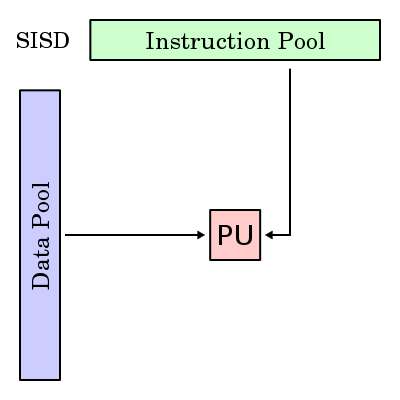
\includegraphics[width=150pt]{images/SISD.png}			
		}
		\subfigure[Diagrama de SIMD.]{
			\label{simd}	
			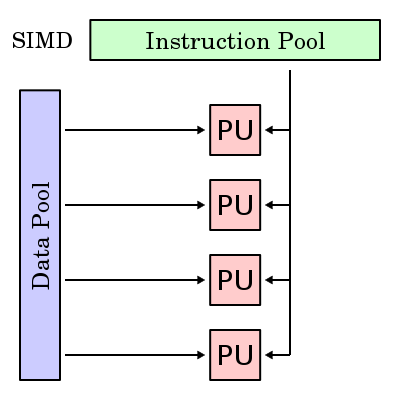
\includegraphics[width=150pt]{images/SIMD.png}			
		}
		\label{flynDiagram}
		\\
		\subfigure[Diagrama de MISD.]{
			\label{misd}	
			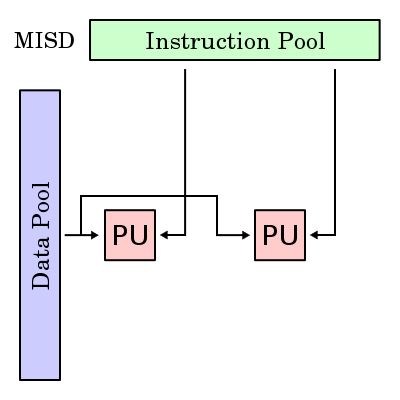
\includegraphics[width=150pt]{images/MISD.png}			
		}
		\subfigure[Diagrama de MIMD.]{
			\label{mimd}	
			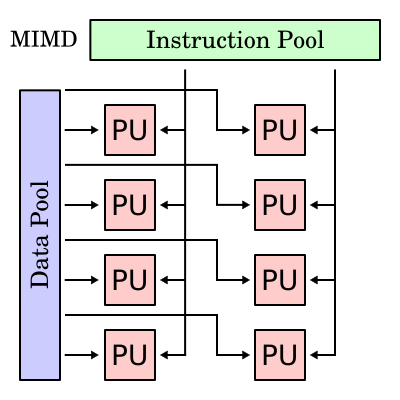
\includegraphics[width=150pt]{images/MIMD.png}			
		}
		\caption{Taxonomia de Flynn}
	\end{figure}	

\subsection{Resolución de problemas paralelos}

Cuando tenemos un problema que requiere una gran capacidad de cómputo, ya sea por una gran cantidad de datos de entrada o por una gran
complejidad en sus operaciones, podemos optar solucionarlo mediante el desarrollo de algoritmos paralelos. El primer paso para el diseño de
un algoritmo paralelo consiste en descomponer el problema principal en problemas más pequeños o subproblemas para que luego sean asignados a
cada procesador y puedan ser ejecutados de manera independiente y simultánea.

No siempre es una buena decisión partir de un algoritmo secuencial intentando ``paralelizar'' la aplicación, sino que en ciertas ocasiones
es necesario diseñar un nuevo algoritmo que, seguramente, será muy diferente al secuencial.
Entre las descomposiciones mas conocidas se encuentran:

    \begin{description}
     \item[Descomposición de dominio o paralelismo de datos] consiste en descomponer los datos de entrada de
un programa paralelo en porciones más pequeñas e indivisibles de tal manera que posean aproximadamente el mismo tamaño. Cada una de estas
porciones son asignadas a un procesador para su posterior ejecución. Se puede relacionar al paralelismo de datos con el modelo \textbf{SIMD}
ya que permite mantener un único flujo de instrucciones.
     \item[Descomposición funcional] se basa en la división del programa principal en subtareas mas pequeñas donde cada una de éstas son
asignadas y ejecutadas de manera independiente por cada procesador. En muchos casos, el número de subtareas obtenidas puede ser mayor a la
cantidad de procesadores con los que se cuenta. \\
Este tipo de descomposición se implementa siguiendo un paradigma maestro-esclavo donde existe un proceso maestro que se encarga de enviar
subtareas a los procesos  esclavos. Cuando uno de éstos últimos termina su computación, los resultados se envían al proceso maestro el cual
nuevamente le asigna una nueva subtarea a procesar. Se prosigue de ésta manera hasta agotar las subtareas pendientes.
    \end{description}

\subsection{Paradigmas de programación paralela}

Los paradigmas de programación no están totalmente ligados a las arquitecturas paralelas, pero si estrechamente relacionado. Podríamos decir
que cada arquitectura de computación paralelas justifica esta relación haciendo uso de dichos paradigmas. Es por eso que un determinado
paradigma puede ser más eficiente que otros al programar  sobre determinadas arquitecturas paralelas. Existen dos tipos de paradigmas
principalmente utilizados para la programación paralela:

    \begin{description}
     \item[Memoria compartida] Se ve a los programas como una colección de procesos que pueden acceder a variables locales y a variables
globales almacenadas en un espacio de memoria compartido entre las diversas unidades de procesamiento. Cada proceso accede a dicha memoria
compartida a través de lecturas asíncronas.\\
Este paradigma, como bien lo indica su nombre, es apropiado para el desarrollo de aplicaciones sobre arquitecturas de memoria compartida,
aunque también puede ser utilizado para el desarrollo de aplicaciones para arquitectura distribuida, simulando un espacio de memoria
compartido.
    \item[Paso de mensajes] es una técnica empleada para aportar sincronización entre procesos y permitir la exclusión mutua de manera
similar a como se hace con los semáforos, monitores, etc. Su principal característica es que no precisa de memoria compartida, por lo que es
muy importante en la programación de sistemas distribuidos. Los elementos principales que intervienen en el paso de mensajes son: el proceso
que envía, el que recibe y el mensaje.
    \end{description}

\subsection{Balanceo de carga}

Un aspecto fundamental que hay que tener en cuenta a la hora de desarrollar un programa paralelo es el \textit{balanceo de carga}.

Ésta es una metodología para distribuir equitativamente los trabajos a través de múltiples computadoras, clusters, redes de trabajos,
discos, o todo aquello que conforme el sistema paralelo utilizado, de tal manera que se pueda asegurar el uso y distribución óptima de los
recursos y poder maximizar la salida, minimizar el tiempo de respuesta y evitar sobrecargas. El servicio de \textit{balanceo de carga}
usualmente lo proveen programas dedicados o dispositivos de hardware\cite{buyya99}.

El equilibrio de carga es comúnmente utilizado para realizar comunicaciones internas en clusters o para implementar algoritmos de
planificación en sistemas operativos.

\subsection{Etapas de diseño}

Las etapas de diseño de aplicaciones paralelas podrían resumirse entonces como sigue:

\begin{itemize}
 \item Identificar el trabajo que puede realizarse en paralelo.
 \item Diseñar la división y unificación del trabajo y datos entre los procesadores.
 \item Resolver el acceso a los datos, las comunicaciones entre procesos y las sincronizaciones.
 \item Asignar recursos de cómputo a los procesos que se ejecutarán en paralelo.
\end{itemize}


\section{FuD}
\label{sec:fud}

FuD es un framework para la distribución de procesos, o bien, un framework para la implementación de aplicaciones distribuidas\cite{clus09}.
FuD no depende del problema a implementar y no fuerza a usar un modelo de comunicación particular ni restringue a cualquier disposición de
nodos de procesamiento con que se cuente. Por lo tanto, las aplicaciones pueden ejecutarse en cluters heterogéneos y dinámicos.

Este framework provée una base para pequeños y medianos proyectos que necesitan manejar grandes conjuntos de datos y particularmente con
gran demanda de independencia de procesamiento con bajos requerimientos de comunicación.

FuD se divide entre aplicación servidor y cliente organizado en tres capas, cada una con una responsabilidad clara. La comunicación entre
las mismas es limitada estrictamente, cada una ellas tiene solo un punto de comunicación.
Las capas y sus responsabilidades son las siguientes:

\begin{figure}[!ht]
\begin{center}
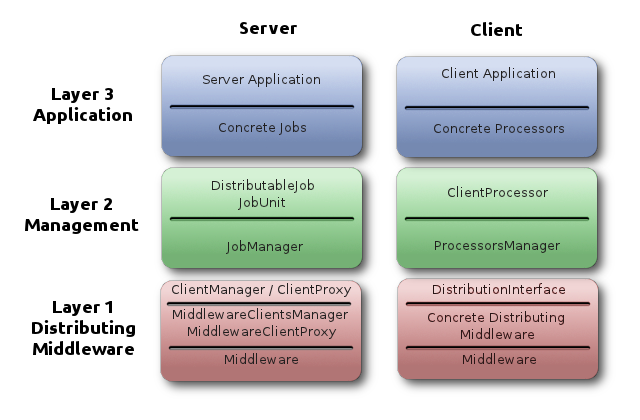
\includegraphics [width=300pt]{images/FuD-AbstractLayers.png}
\label{fud_layers}
\end{center}
\caption{Diseño de FuD.}
\label{fud-layers}
\end{figure}

\begin{description}
	\item[Capa de aplicación (L3)] Esta capa proporciona componentes que describen el problema a resolver, tanto en lo que respecta a los
            algoritmos y los datos utilizados. En el lado del servidor reside la aplicación principal, la distribución de la estrategia y
            los componentes de datos. En el lado del cliente, sólo una aplicación de los métodos para hacer los cálculos correspondientes en
            las unidades de trabajo.	
	\item[Capa de manejo de trabajo (L2)] La responsabilidad de esta capa es manejar los trabajos, que pueden ser divisibles o atómicos.
            Registran trabajos distribuibles concretos y genera unidades de trabajo que son pasados a la capa subyacente para su
            procesamiento y una vez obtenido el resultado correspondiente informa a la capa superior la finalizacion del trabajo y la
            comunicación de los resultados.
	\item[Capa de comunicación (L1)] En el lado del servidor, el registro y estado de clientes se maneja en esta capa. En ambos lados hay
            una subcapa constante que son las interfaces del middelware mientras que las implementaciones concretas estan en otra subcapa
            variable (Por ejemplo, BOINC\footnote{Berkeley Open Infrastructure for Network Computing. http://boinc.berkeley.edu} o
            MPI\footnote{An API specification for communication: http://www.mpi-forum.org/docs} ).
			
\end{description}


\section{Recursión}

En el sentido más amplio de la palabra, \textbf{recursión} (o recurrencia, o recursividad) es la forma en la cual se especifica un proceso
basado en su propia definición. Dicho de otra forma, es el proceso de repetir cosas de una manera \textit{auto-similar}, propiedad de un
objeto en el que el todo es exacta o aproximadamente similar a una parte de sí mismo.
La recursión, en ciencias de la computación, es un método para resolver problemas computacionales donde la solución depende de las
soluciones de instancias más pequeñas del mismo problema\cite{conmath94}.

\begin{quote}
    \textit{``El poder de la recursión, evidentemente, radica en la posibilidad de definir un conjunto infinito de objetos con una
    declaración finita. De la misma manera, un número infinito de cálculos puede ser descrito por un programa recursivo finito, aunque este
    programa no contenga repeticiones explícitas.''}\cite{algdatpro76}
\end{quote}

En computación el artefacto de la recursión es el \textit{algoritmo recursivo}. Estos algoritmos tienen una importancia fundamental e
indispensable en prácticamente todas las áreas en el campo de la informática. Para muchos problemas, el uso de la recursividad permite
resolver problemas complejos mediante algoritmos concisos, fáciles de comprender y eficientes (desde el punto de vista algorítmico).

En su forma más simple, la recursividad es el proceso de dividir el problema en uno o más subproblemas, que son idénticos en estructura al
problema original y luego la combinación de las soluciones a estos subproblemas para obtener la solución al problema original. Pero en
general podemos identificar tres casos especiales de esta técnica de diseño:
\begin{enumerate}
    \item   \textbf{Inducción} (o tail recursion).
    \item   Subproblemas sin superposición, usando \textbf{divide \& conquer}.
    \item   Subproblemas con superposición con redundantes invocaciones a subproblemas, lo que permite intercambiar espacio por tiempo. Se
            usa la técnica de \textbf{programación dinámica}.
\end{enumerate}

Los casos con números superiores incluyen a los de números más bajos. En los primeros dos casos no se requiere espacio adicional para llegar
a la solución. La tercera clase, sin embargo, da la posibilidad de solucionar eficientemente muchos problemas que a primera vista parecen
consumir mucho tiempo, debido a los repetidos cómputos que se realizan sin esta técnica\cite{alsuwaiyel98}.

Cabe aclarar que, el alcance de este trabajo abarca sólo las dos primeras técnicas. Aún así, el último caso es desarrollado también, a
modo de ejemplo de técnica no aplicable en este proyecto.

\subsection{Inducción}

En esta sección veremos a la inducción como una técnica para el desarrollo de algoritmos, en pocas palabras: la idea de inducción en pruebas
matemáticas es llevada al plano computacional obteniendo, así, diseño de algoritmos eficientes.

Para entender esta técnica vamos a considerar un problema de tamaño $n$, el cual normalmente representa el número de objetos (o partes) de
un problema. Cuando buscamos una solución para un problema en particular, algunas veces es más fácil comenzar solucionándolo con un
parámetro mas chico, $n-1$, $n/2$, etc, y extender esta solución para incluir los $n$ objetos. Esta forma de resolver problemas esta basada
en la muy conocida técnica de prueba: \textbf{inducción matemática}. Básicamente, dado un problema de parámetro $n$, diseñar un algoritmo
por inducción esta basado en el hecho de que si sabemos resolver el problema cuando tiene un parámetro menor a $n$, esto es llamado la
\textit{hipótesis inductiva}, entonces nuestra tarea se reduce a extender la solución para incluir a todos los objetos, llegando así al
parámetro $n$.

Este método puede ser generalizado para alcanzar todas las técnicas de diseño de algoritmos recursivos incluyendo las de divide \& conquer y
programación dinámica, sin embargo, estas tienen diferentes características que serán vistas en las próximas dos secciones.

En resumen, podemos decir que otras técnicas de programación tienen una estrecha relación con la \textit{inducción} pero vamos a darle ese
nombre sólo a los algoritmos que usen estrategias basadas \textit{claramente} de inducción matemática, a aquellos algoritmos que usualmente
sólo tienen una llamada recursiva, y son comúnmente llamados \textit{tail recursion}. Estos, en la mayoría de los casos, pueden ser
convenientemente convertidos a algoritmos iterativos.

Una ventaja de esta técnica (y de todos los algoritmos recursivos en general) es que la prueba de corrección del algoritmo diseñado es
naturalmente visto como su descripción, y por lo tanto una simple prueba inductiva puede ser fácilmente construida si se
desea\cite{alsuwaiyel98}.


\subsection{Divide \& Conquer} \label{divideandconquer}

Como dijimos anteriormente, podemos encontrar casos especiales de esta técnica de diseño llamada recursión, y una de ellas es la de resolver
recursivamente problemas que tienen subproblemas sin superposición entre ellos, o sea, problemas en los que no se comparten mismas
soluciones para subproblemas generados. Esto es a lo que se le llama en inglés \textit{Nonoverlapping subproblems}, y este tipo de problemas
puede ser naturalmente resuelto por la conocida técnica de \textbf{Divide \& Conquer}\cite{levitin06}.

\begin{quote}
    \begin{flushright}
        \textit{``Divide et vinces'' (Divide y vencerás),\\Julio César.}
    \end{flushright}
\end{quote}

Esta frase célebre nos conduce a una buena estrategia recursiva para resolver problemas que se puedan dividir en subproblemas más
sencillos.

% Alsuwaiyel page 175
En ciencias de la computación, el término ``\textit{divide y vencerás}'' hace referencia a una poderosa técnica de diseño de
algoritmos utilizada para resolver una amplia variedad de problemas. En su forma más simple, un algoritmo \textit{divide \& conquer} divide
un problema en una serie de subproblemas (en la mayoría de los casos 2), luego resuelve de forma recursiva cada uno de ellos por separado, y
por último, combina las soluciones de los subproblemas para obtener la solución al problema original\cite{alsuwaiyel98}.\\

% Cormen page 29
Según el libro \cite{cormen09}, el paradigma \textit{divide \& conquer} involucra tres pasos en cada nivel de la recursión:
\begin{itemize}
    \item   \textbf{Dividir} el problema en un numero de subproblemas.
    \item   \textbf{Conquistar} los subproblemas, resolviéndolos recursivamente. Por más que el tamaño de los subproblemas sean lo
            suficientemente pequeños, sólo se deben resolver de una manera directa.
    \item   \textbf{Combinar} las soluciones de los subproblemas en la solución del problema original.\\
\end{itemize}

% Skiena page 147
\begin{flushleft}
    \textbf{Relación de recurrencia}
\end{flushleft}
 
Como sabemos, una relación de recurrencia, que pasado al plano computacional se puede ver como un algoritmo recursivo, es una ecuación
que está definida en términos de ella misma. Por ejemplo, los \textit{números de Fibonacci}\cite{sigler03} están descritos por la relación
de recurrencia $F_n = F_{n-1} + F_{n-2}$. Esencialmente, las relaciones de recurrencia proporcionan una manera de analizar las estructuras
recursivas, tales como los algoritmos.

La función para el tiempo de ejecución de un algoritmo \textit{divide \& conquer} esta basado en los tres pasos del paradigma básico,
mencionados anteriormente. Sea $T(n)$ el tiempo en que se ejecuta un problema de tamaño $n$. Si el tamaño del problema es lo suficientemente
pequeño, como por ejemplo $n \leq c$ para una constante $c$, la solución trivial toma un tiempo constante, denotado por $\Theta(1)$.
Supongamos que la división del problema se obtiene en $a$ subproblemas, y cada uno de ellos es $1/b$ el tamaño del original. Si tomamos a
$D(n)$ como el tiempo para dividir el problema en subproblemas y que $C(n)$ es el tiempo para combinar las soluciones de los subproblemas en
la solución del problema original, obtenemos la siguiente función $T(n)$:\\

\[ T(n) = \left\{ \begin{array}{ll}
         \Theta(1) & \mbox{if $n \leq c$ },\\
         aT(n/b) + D(n) + C(n) & \mbox{otherwise} \end{array} \right.
\]

La figura \ref{recursion_tree} muestra el árbol de recursión asociado con un típico $T(n)$ de un algoritmo divide y vencerás. Cada problema
de tamaño $n$ se descompone en un problema de tamaño $n/b$. Cada subproblema de tamaño $k$ toma un tiempo $O(f(k))$ para ocuparse de su
interior, entre la partición y luego su fusión. El tiempo total para el algoritmo es la suma de los costos internos, mas el
\textit{overhead} de construir el árbol de recursión. La altura de este árbol es $h = \log_b n$ y el número de hojas $a^h = a^{\log_b n}$,
que se simplifica en $n^{\log_b a}$ con un poco de manipulación algebraica.

\begin{figure}[!ht]
\begin{center}
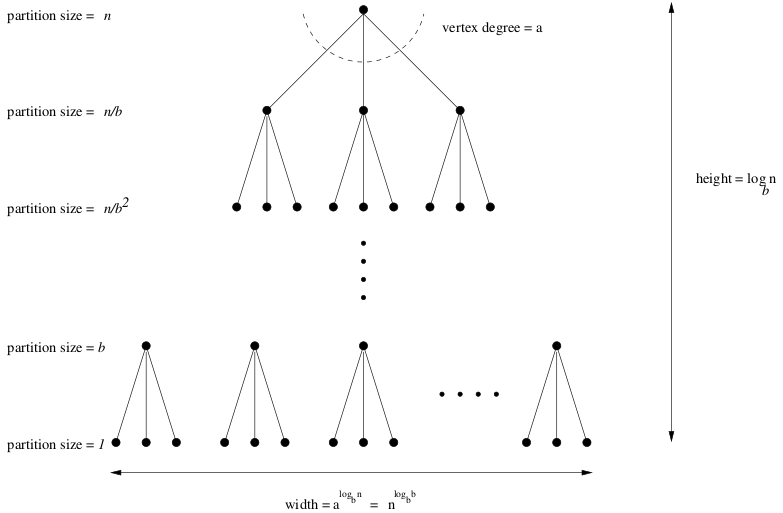
\includegraphics[width=400pt,height=262pt]{images/recursion-tree.png}
\end{center}
\caption{Árbol de recursión resultante de descomponer cada problema de tamaño $n$ en subproblemas de tamaño $n/b$.}
\label{recursion_tree}
\end{figure}

% Ejemplo Fibonacci
Siguiendo con el ejemplo de la sucesión de Fibonacci, su definición recursiva sería la siguiente:
\begin{equation} \label{def-fib} \end{equation}
\[ Fib(n) = \left\{ \begin{array}{ll}
         1 & \mbox{if $n = 1$ or $n = 2$ },\\
         Fib(n-1) + Fib(n-2) & \mbox{if $n \geq 3$} \end{array} \right.
\]
Dada esta definición, es fácil escribir un programa recursivo para computar el número de Fibonacci $N$.
Esta versión recursiva tiene la ventaja de ser concisa, fácil de escribir, de depurar y, sobre todo, su abstracción es clara. Hay una clase
rica de algoritmos recursivos y, en muchos casos, un complejo algoritmo se puede escribir sucintamente con el uso de la recursividad.\\

% Skiena page 147
Problemas más pequeños nos permiten centrarnos en detalles que se pierden cuando se está estudiando al problema por completo. Un algoritmo
recursivo comienza a ser evidente cuando se puede dividir el problema en partes más pequeñas del mismo tipo de problema. Para un
procesamiento paralelo eficaz se requiere una descomposición de trabajos en, al menos, tantas tareas como procesadores, y este es un tema
cada vez más importante debido al advenimiento de \textbf{cluster computing} y los procesadores multinúcleo\cite{skiena08}.

% Alsuwaiyel page 155
Como conclusión vemos que, las ventajas más atractivas de algoritmos divide \& conquer son: la concisión, la facilidad de comprensión y
ejecución, y lo más importante es que se pueden hacer, de manera fácil, pruebas de inducción para demostrar la corrección de este tipo de
algoritmos.


\subsection{Programación Dinámica}

% Common knowledge and wikipedia
Como bien sabemos, la \textit{programación dinámica} es una de las técnicas de programación mas usadas para resolver problemas en los
cuales sus subproblemas no son independientes, o sea, que \textit{comparten} soluciones comunes, a lo cual llamamos \textit{subproblemas
superpuestos}. Cada subproblema se resuelve sólo una vez y se guarda la respuesta en una tabla, evitando así el trabajo de volver a
calcular la respuesta cada vez que se encuentra el subproblema. 

La programación dinámica es típicamente utilizada en \textit{problemas de optimización}. En este tipo de problemas puede haber muchas
soluciones posibles. Cada solución tiene un valor, y queremos encontrar una solución con el valor óptimo (mínimo o máximo). Llamamos
a esta solución \textbf{una} solución óptima al problema, a diferencia de \textbf{la} solución óptima, ya que puede haber varias soluciones
que permitan alcanzar el valor óptimo\cite{cormen09}.

Más específicamente, la programación dinámica es aplicada a problemas con \textit{subestructura óptima}. Un problema se dice que tiene
subestructura óptima si una solución óptima se puede construir de manera eficiente de las soluciones óptimas para sus subproblemas. Por
ejemplo, el camino más corto entre dos vértices de un grafo se puede encontrar calculando primero el camino más corto al objetivo desde
todos los vértices adyacentes al de partida, y después usando estas soluciones para elegir el mejor camino de todos
ellos\cite{bellman10}.\\

% Alsuwaiyel page 155
Pero... ¿Qué tiene que ver recursión con programación dinámica?
% 
En esta técnica de diseño, la recursividad es solamente utilizada para modelar la solución del problema, como enfoque de la solución. Luego,
este modelo recursivo se convierte, en la mayoría de los casos, en un eficiente algoritmo iterativo en contraste con las redundantes
llamadas que hace la recursión\cite{alsuwaiyel98}.

% Skiena page 285
De hecho, la programación dinámica es una técnica eficiente para la implementación de un algoritmo recursivo mediante el almacenamiento de
resultados parciales. El truco está en ver si el \textit{ingenuo} algoritmo recursivo calcula el mismo subproblema una, y otra, y otra vez.
Si es así, el almacenamiento de la respuesta para cada subproblema en una tabla para luego buscar, en lugar de volver a calcular, puede dar
lugar a un algoritmo eficiente. Comienza con un algoritmo o definición recursiva. Sólo una vez que tenemos un algoritmo recursivo correcto,
ahora lo que nos preocupa es acelerarlo mediante el uso de una matriz de resultados.

La programación dinámica es generalmente el método adecuado para problemas de optimización combinatoria en objetos que tienen inherentemente
un orden de izquierda a derecha entre los componentes. Entre los objetos de-izquierda-a-derecha se incluyen: cadenas de caracteres, árboles
con raíces, polígonos, y secuencias de números enteros. La programación dinámica se aprende mejor mediante el estudio cuidadoso de ejemplos
hasta que las cosas comienzan a hacer un ``click'' en nuestra cabeza\cite{skiena08}\cite{moshe10}.\\


\begin{flushleft}
    \textbf{Construcción de un algoritmo dinámico}
\end{flushleft}
% Pasos para desarrollar un algoritmo con la tecnica de programacion dinamica. Cormen 277.
La construcción de un algoritmo mediante esta técnica puede ser dividida en cuatro pasos:
\begin{enumerate}
    \item   Caracterizar la estructura de una solución óptima. 
    \item   Recursivamente, definir el valor de una solución óptima.
    \item   Computar el valor de una solución óptima en un orden \textit{bottom-up} (de abajo hacia arriba en el árbol de recursión).
    \item   Construir una solución óptima a partir de la información computada.
\end{enumerate}
Los pasos 1, 2 y 3 son la base de una solución de programación dinámica a un problema. El paso 4 puede omitirse sólo si el valor de una
solución óptima es necesario. Cuando se realiza el paso 4, a veces se mantiene información adicional durante el cálculo del paso 3 para
facilitar la construcción de una solución óptima\cite{cormen09}.\\

\begin{flushleft}
    \textbf{Ejemplo: Fibonacci}
\end{flushleft}
% Seguir con ejemplo Fibonacci comparando con algoritmo recursivo. Skiena 286 & Alsuwaiyel 217.
Como planteamos en la sección \ref{divideandconquer} ``Divide \& Conquer``, los números de Fibonacci, descritos por su definición
recursiva expresada anteriormente en ecuación \ref{def-fib}, generan una secuencia de números naturales en el cual cada número es la suma
de los dos números precedentes (salvo los dos primeros que se definen como caso base). El principio de la secuencia es:
\begin{center}
    $F(0)=0, F(1)=1, F(2)=1, F(3)=2, F(4)=3, F(5)=5, F(6)=8, ....$
\end{center}

La ejecución del algoritmo recursivo para computar el enésimo número de Fibonacci se refleja en su árbol de recursión, como se ilustra en la
figura \ref{recursion_tree_fib}. Este árbol es evaluado de una manera \textit{depth-first}, al igual que todos los algoritmos recursivos.

\begin{figure}[!ht]
\begin{center}
\begin{tikzpicture}[level/.style={sibling distance=70mm/#1}]
    \tikzstyle{every node}=[none]
    \node {$F(5)=5$}
        child {
            node {$F(4)=3$}
            child {
                node[rectangle,draw,fill=blue!12]{$F(3)=2$}
                child {
                    node[rectangle,draw,fill=red!12]{$F(2)=1$}
                    child {
                        node {$F(1)$}
                        child {node[circle,draw]{$1$}}
                    }
                    child {
                        node {$F(0)$}
                        child {node[circle,draw]{$0$}}
                    }
                }
                child {
                    node {$F(1)$}
                    child {node[circle,draw]{$1$}}
                }
            }
            child {
                node[rectangle,draw,fill=red!12]{$F(2)=1$}
                child {
                    node {$F(1)$}
                    child {node[circle,draw]{$1$}}
                }
                child {
                    node {$F(0)$}
                    child {node[circle,draw]{$0$}}
                }
            }
        }
        child {
            node[rectangle,draw,fill=blue!12]{$F(3)=2$}
            child {
                node[rectangle,draw,fill=red!12]{$F(2)=1$}
                child {
                    node {$F(1)$}
                    child {node[circle,draw]{$1$}}
                }
                child {
                    node {$F(0)$}
                    child {node[circle,draw]{$0$}}
                }
            }
            child {
                node {$F(1)$}
                child {node[circle,draw]{$1$}}
            }
        }
    ;
\end{tikzpicture}
\end{center}
\caption{Árbol de recursión para computar el quinto número de Fibonacci.}
\label{recursion_tree_fib}
\end{figure}

Tenga en cuenta que $F(3)$ (en azul) se calcula en ambos lados del árbol de recursión y $F(2)$ (en rojo) se calcula tres veces en este
pequeño ejemplo. El peso de todas estas redundancias se hace evidente cuando se ejecuta el programa. Sólo nos queda imaginarnos cuántos
minutos tarda un programa para calcular los primeros 45 números de Fibonacci. Esta solución recursiva toma un tiempo exponencial, por lo que
se hace inmanejable a valores altos de entrada.

Pero... Que pasa si calculamos sólo una vez cada número de Fibonacci ?\\Esto es, en el ejemplo, para calcular $F(5)$, computamos por única
vez $F(4)$, $F(3)$ y $F(2)$ (con  $F(0)$ y $F(1)$ como casos base), con lo que nos alcanza para calcular el resultado final. Esto es
justamente lo que logra la técnica de \textbf{programación dinámica}, en la cuál evaluamos los números de Fibonacci de menor a mayor y
almacenamos todos los resultados, y de esta manera sabemos que tenemos $F(i-1)$ y $F(i-2)$ listos cada vez que necesitamos calcular $F(i)$.
La linealidad de este algoritmo es evidente, cada uno de los valores de $n$ se calcula como la simple suma de dos números enteros, lo que
nos da como total: $O(n)$ en tiempo y espacio.

% To add:
% Eleccion del nombre "programacion dinamica". Stuart Dreyfus paper. \cite{Dreyfus:2002:RBB:767815.769382}
% Multi-stage allocation process. Bellman book.


\subsection{Divide \& conquer vs. programación dinámica}
% Recursion vs programacion dinamica, arbol con repeticion. Papadimitriou 5.

Como dijimos anteriormente, la técnica de programación dinámica no usa generalmente algoritmos recursivos, sino que usa la noción de
recursividad solamente para modelar la solución del problema, o sea, como enfoque de la solución.

Pero: ¿ Por qué la recursión funciona tan bien con divide \& conquer ? El punto clave es, que en esta técnica, un problema es expresado en
términos de subproblemas \textbf{sustancialmente} más pequeños, digamos la mitad de tamaño. Por ejemplo, el algoritmo \textit{mergesort}
ordena un arreglo de tamaño $n$ haciéndolo recursivamente con dos subarreglos de tamaño $n/2$. Debido a esta fuerte caída en el tamaño del
problema, el árbol de recursión completo sólo tiene profundidad logarítmica y un número polinómico de nodos.

Por el contrario, en un diseño de programación dinámica habitual, un problema se reduce a subproblemas que son sólo \textbf{ligeramente} más
pequeños, por ejemplo, $L(j)$ se resuelve con $L(j-1)$. Así, el árbol de recursión completo por lo general tiene una profundidad polinómica
y un número exponencial de nodos. Sin embargo, resulta que la mayoría de estos nodos se repite, por lo que indica que no hay demasiados
subproblemas distintos entre ellos. Luego, la eficiencia es obtenida enumerando explícitamente los distintos subproblemas y resolviéndolos
en el orden correcto\cite{algorithms06}.

\section{Lenguaje \cpp}

\cpp{} es un lenguaje de programación de propósito general con tipado estático, de forma libre, compilado y orientado a objetos. Es
considerado como un lenguaje de nivel intermedio, ya que comprende una combinación de características de lenguajes tanto de alto como de
bajo nivel. Fue desarrollado por Bjarne Stroustrup a partir de 1979 en los Laboratorios Bell como una mejora del lenguaje de programación
\textbf{\textit{C}} y originalmente fue llamado ``C con clases''. La referencia más completa para el lenguaje se puede encontrar en el gran
libro del mismo Stroustrup\cite{cplusplus}.

\cpp{} fue elegido como el lenguaje de implementación ya que permite el uso de técnicas orientadas a objetos y produce código máquina muy
eficiente, lo que da como resultado programas rápidos. \cpp{} también ofrece una gran cantidad de bibliotecas para elegir, permitiendo a
los programadores concentrarse en el programa en cuestión y no en reimplementar tipos abstractos de datos conocidos.
